\chapter{On Algorithms for Building and Sampling Disordered Crystal States}
\label{ch:iceXI}

TODO: FIX ICE IH - I$_{h}$
As discussed in the introduction, ice I$_{h}$ modeling comes with computational challenges. 
The problem of generating a random proton-disordered crystal with only ordered pseudorandom tools presents as a technical impossibility. 
However, through the usage of averages and distributions, it is possible to generate a pseudorandom proton-disordered crystal that behaves similar to a truly random proton-disordered crystal.


\section{Ice Annealing}

EACH SUBSECTION: DEFINITION OF TERMS

\subsection{Bernal - Fowler Ice Rules}

Citation! \cite{BFIceOG}

There have been many works published on this topic, so I will have no problem obtaining a cohesive review. I plan to include the various forms of ice and focus on I$_{h}$ and XI. This includes differences between the two in prevalence, environment, and synthesis (is synthesis the correct term here?). 

I expect to focus on many thermodynamic properties and to focus on entropy as a driving force of difference in the modeled system. I will include publications of the effort to model a truly proton-disordered system and focus on the computational aspect. 

\subsection{Structures of Ice}

Ice contains many structures.
These structures are typically orthorhombic, which means rectangular at non-90º angles.
They can also be hexagonal, cubic, else. 
These different structures form based on temperature and pressure. 
Ice I$_{h}$ is the most prevalent form of ice found normally on earth, forming at pressures around 1 atm and temperatures around 0ºC. (source needed?).

More detail on ice I$_{h}$.

More detail on ice XI.

\subsection{Residual Entropy of Ice I$_{h}$ and Ice XI}

Residual entropy is a thermodynamic property that greatly differs between ice I$_{h}$ and XI. 
In general, entropy can be calculated for a system of $N$ molecules as $S = Nk\ln(w)$, where $k$ is the Boltzmann constant and $w$ is the number of real microstates corresponding to any macrostate.
Residual entropy differs in calculation from entropy in that it generally refers to the entropy of a crystal near zero kelvin. 
Linus \cite{PaulingIce} described the $w$ of very low temperature crystals to approach the number of orientations possible for each molecule with consideration to immediate neighbors. 
Since ice I$_{h}$ is a 

For a proton-disordered ice I$_{h}$ crystal, $w$ becomes $\frac{x}{2^{4}}$ where $x$ is the number of acceptable orientations within the crystal.

\subsection{Hydrogen Bond Defects in Ice Crystals}

Speak here about defects and how they quantitatively harm stability and why the defects need to be reduced in general ice I$_{h}$ structures.

\subsection{Literature Review on Relevant Works}

words????


\section{Framing the Problem}
While ice I$_{h}$ is known as the most common form of ice found on the planet, it is much more difficult to generate than an ice XI lattice. 
The ease of generation of an ice XI structure stems from the repetition of a unit cell with consistent layering and orientation throughout the crystal lattice. 
All protons and lone pairs are ordered in a consistent manner that produce proper hydrogen bonds. 
As such, lattice defects do not naturally arise in the computational structure without running a simulation with sufficient energy to perturb the system.

With ice I$_{h}$ crystals, the proton-disordered form introduces entropy by way of rotational disorder. 
As the protons and lone pairs are no longer consistently ordered, hydrogen bonds may no longer form properly at all interaction sites. 
The interaction of proton with proton or lone pair with lone pair are not hydrogen bonds and are considered defects in the lattice. 
An ice structure of randomly oriented molecules without consideration of hydrogen bonds will likely produce defects at many interaction sites across the lattice and weaken the integrity of the system, leading to stability problems while running simulations. 
In generating the crystal, the cause of these defects must be considered and countered effectively.

\section{Method of Generating an Ice I$_{h}$ Crystal}
This approach to generating an ice I$_{h}$ structure involves beginning with a proton- ordered ice XI structure, randomly rotating all water molecules, and then recursively perturbing high-defect regions to reduce the number of overall defects. 
As detailed later, defect thresholds can be adjusted to fit the desired system.
\subsection{Generation of an ice XI crystal}
TODO
This details Dr. Fennell’s method of making an ice XI crystal.
\subsection{Algorithm to rotate water molecules (TODO Code inside?)}
Once the ice XI PDB file has been generated, the next goal is to introduce disorder into the lattice by rotating each water molecule. 
Using the Euler-Rodrigues formula for rotating a three-dimensional point about a vector (detailed below), the water molecule is rotated about the center oxygen atom along the vector of one proton to determine the four spatial potential locations for the two protons. 
These locations are stored in a water object variable for later potential use.
Using a pseudo-random number generator, two of the four location potentials are selected and the PDB file is modified so that the protons occupy those locations. 
The lone pairs are then implied to occupy the two remaining spaces. 
As PDB files do not specify lone pair location, no action is taken to specify this. 
Considering each hydrogen bond location individually, the six possible molecule orientations will yield three orientations each of a proton-occupied or lone pair-occupied location. 
Assuming the rotation is close-enough to random, the probability of occupation by either type is $\frac{3}{6} = \frac{1}{2}$.

While considering each molecule as a whole, (12 distinguishable, 6 indistinguishable)

Because there are six potential orientations of the indistinguishable protons in the four locations each containing three proton-facing and three lone pair-facing orientations, the molecule stands a 2/6 = 1/3 chance of occupying the same orientation after the rotation.
After each molecule is randomly rotated, the molecule likely contains defects at half of all junctions due to the 1/2 chance of any one junction containing either a proton - proton or lone pair - lone pair interaction. 
These defects introduce instability in the lattice and need to be reduced.

\subsubsection{The Euler-Rodrigues Formula}
The Euler-Rodrigues Formula is a method of rotating a three-dimensional object in space by use of four-dimensional quaternions. 
Specifically, it has been used for object rotation in video games for years due to its computational efficiency and analytic accuracy.

https://en.wikipedia.org/wiki/Euler%E2%80%93Rodrigues_formula

\subsubsection{Center of Rotation for Water Molecules}
During the rotation, the center of rotation was set to be the center of the oxygen atom. 
The center of mass of the water molecule is toward the two hydrogens (calculate?). 
The crystal structure isn’t COM-based. 
It’s based on the hydrogen bonds and those line up as an extention from the center of each oxygen atom through each hydrogen atom toward a neighboring oxygen atom. 
Because of that connection, the rotation formula uses the center of the oxygen atom as the basis for molecule rotation.

\subsection{Determining Crystal Defects}
Crystal defects are determined by distance between central oxygen and neighboring oxygen atoms between two water molecules. 
Specifically, the squared distance is calculated to remain computationally efficient. 
This value contains all the pertinent distance information, but squared to prevent the hardware from computing a large number of relatively costly square root calculations. 
If an oxygen atom contains a hydrogen atom in the direction of the neighboring hydrogen atom (or lone pair to lone pair), then a defect is recognized and counted. 
The method utilized to count this is to compare the squared distance between two oxygen atoms with the squared distances between each oxygen atom and neighboring proton of every two neighboring water molecules. 
The neighboring water molecules are determined by calculating the squared distance between oxygen atoms and storing the four closest values.

NEED TO ACTUALLY DO: Recognize edges by wrapping crystal in periodic boundary conditions, recognize neighbor (HOW DO?).

Due to the 50\% likelihood of a defect existing at an interface, the average defect count for all internal water molecules will be near 2. 
This can easily be confirmed by iterating through all internal water molecules, counting the defective interfaces, and dividing the value by 2 times the number of internal molecules.

DefectsAverage,Internal = DefectsInternal (2.1) 2 ∗ NInternalMolecules

\begin{equation}
Defects_{Average, Internal} = \frac{Defects_{Internal}}{2*N_{Internal Molecules}}
\end{equation}

The method allows for a variable average number of defects to be considered and input as a value by the user. Future work may also include a maximum number of defects per molecule.

\subsection{Removing Defects from the Lattice}
This is ongoing, but basically it randomly rotates to reduce the number of defects. 
If impossible, then just move on. 
Also mention the criteria of deciding the number of defects allowed as well as the average defect count (per molecule, not bond pairs). 
Not yet perfect!!!

If the calculated average number of defects is greater than the specified maximum, then actions need to be taken to remove defects without sacrificing the disordered nature of the molecule. 
The method repeats the random rotation mentioned earlier for every molecule and redetermines the defect count for each molecule. 
After each molecule is rotated the new defect count is determined. 
If the defect value is reduced, the rotation is kept. 
If it is equal to or increases the defect prior to the rotation, then the rotation is discarded. 
Once the system has completed iterating through the lattice, the average defect count is redetermined. 
If it remains above the threshold, then the process outlined above is repeated until the criteria is met.

\section{Results of Approach}
Initial results show a successful rotation of water molecules in the lattice to disorder the protons and successfully reclassify the system as ice I$_{h}$. 
An example ice XI lattice of 432 water molecules converted to an ice Ih lattice is shown in figures \ref{fig:iceXI} and \ref{fig:iceIh}.

\begin{figure}
	
	\centering
	
	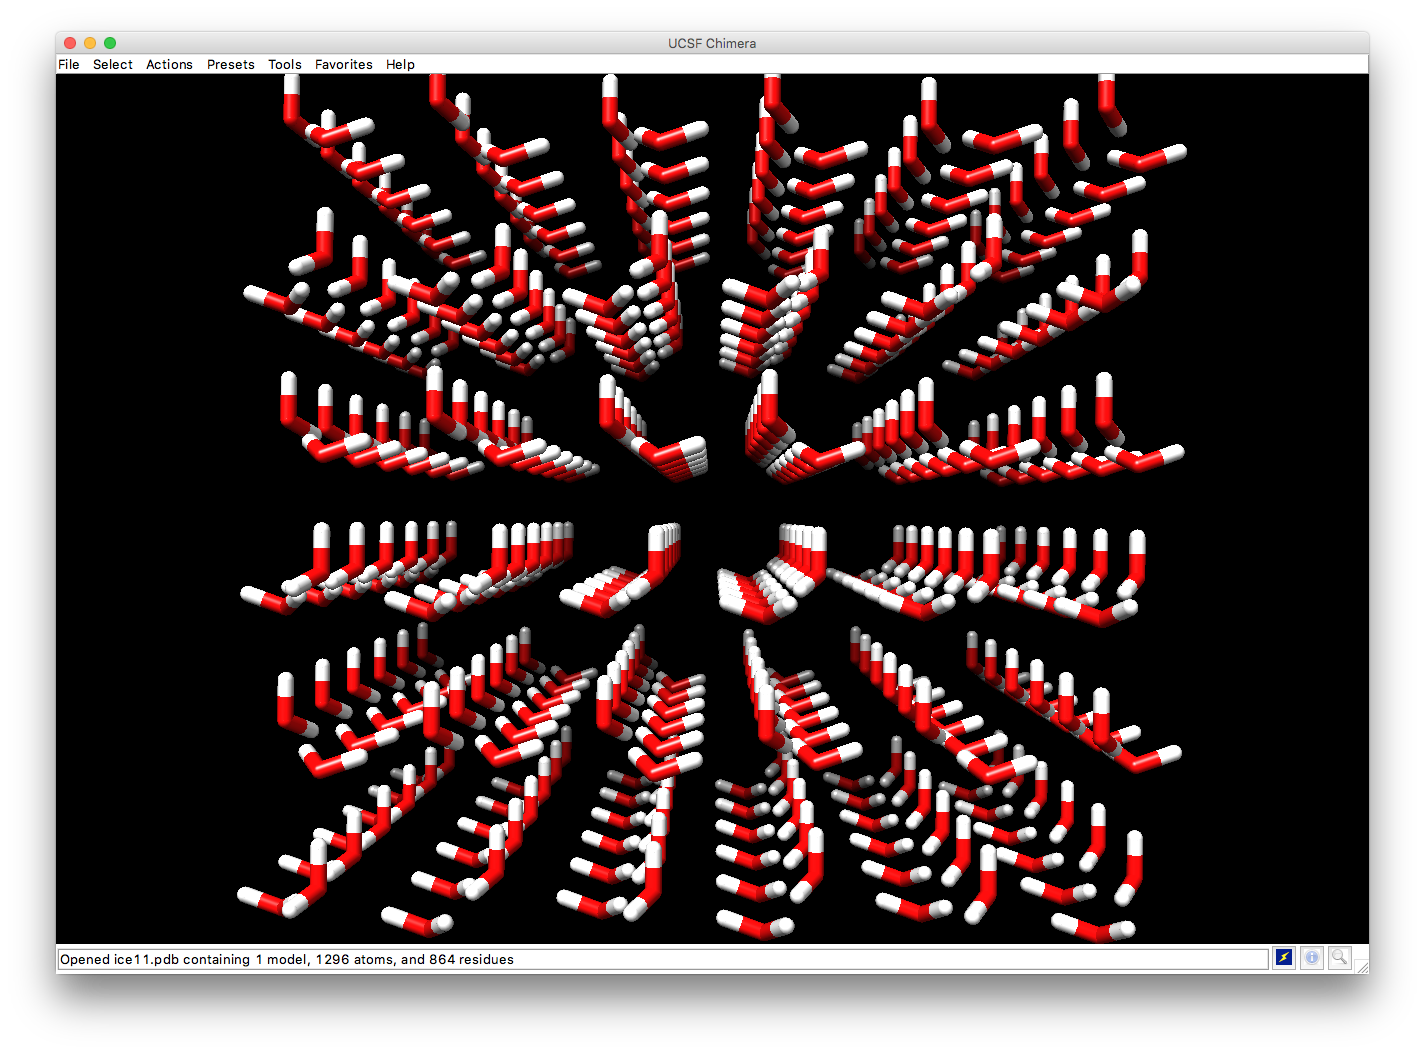
\includegraphics[width=0.75\textwidth]{iceXI.png}
	
	\caption{Ice XI Lattice Before Rotation}
	
	\label{fig:iceXI}
	
\end{figure}

\begin{figure}
	
	\centering
	
	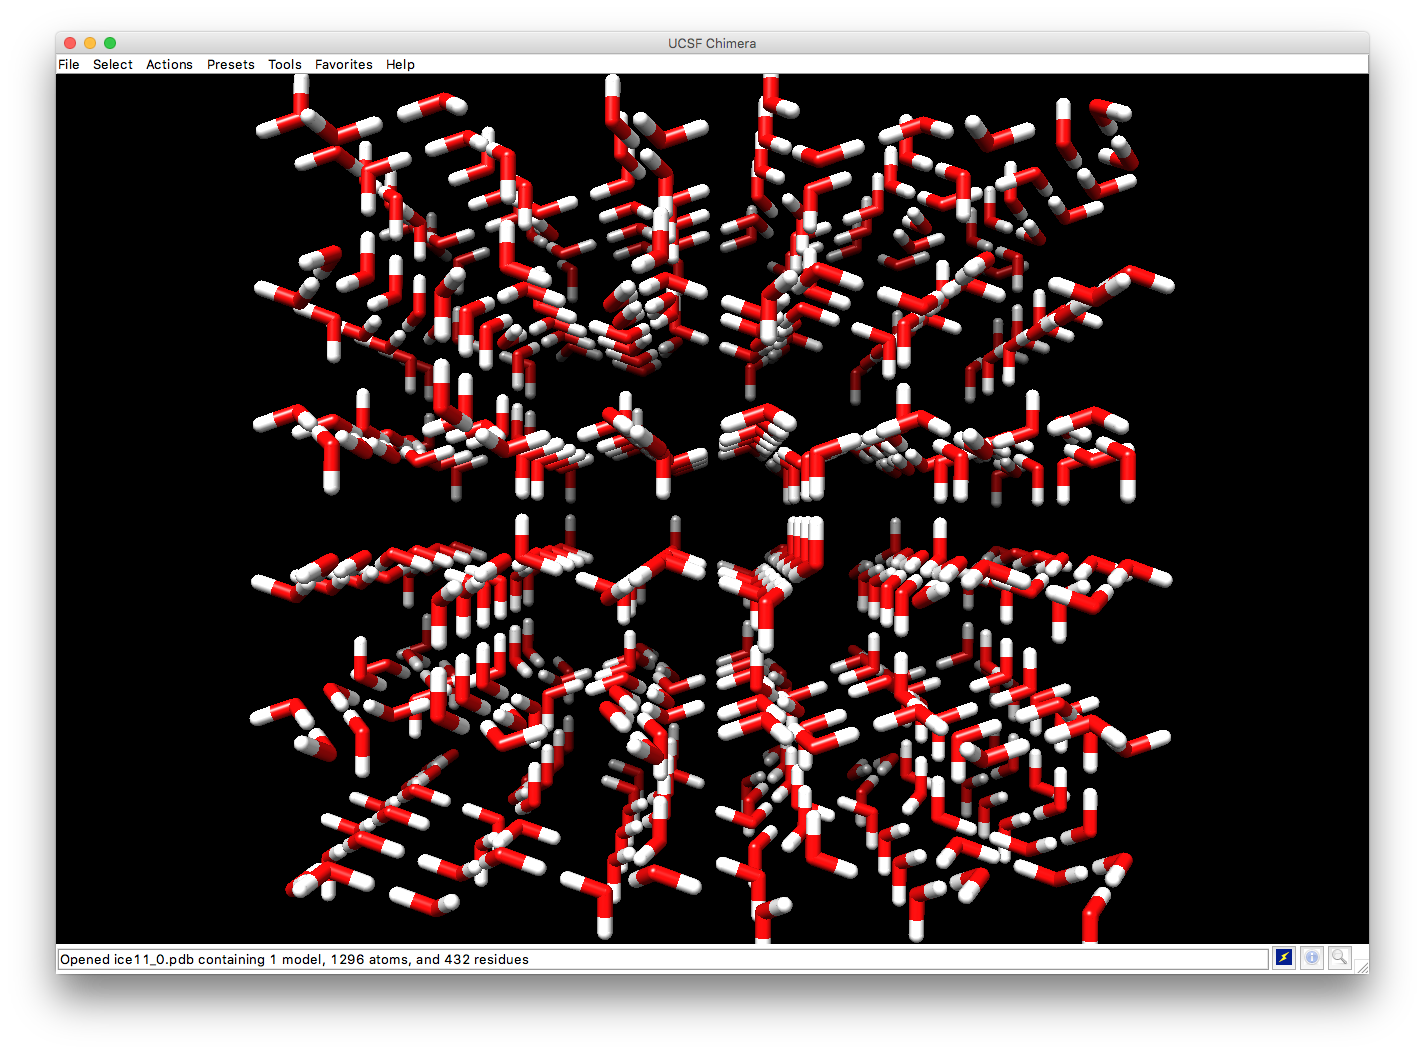
\includegraphics[width=0.75\textwidth]{iceIh.png}
	
	\caption{Ice I$_{h}$ Lattice After Rotation}
	
	\label{fig:iceIh}
	
\end{figure}


\subsection{Difficulties of Method / Known Issues}
Upon closer inspection of figure \ref{fig:iceIh}, there appears to be fragments of order within layers. 
Curiously, multiple regions of repetitive ordered fragments are in different orientations from the original structure. 
Due to the nature of the pseudo-random orientation and the defect removal, molecules rotated to the original orientation may encourage neighboring high-defect molecules to rotate back to their original rotation or to a new pseudo-ordered orientation for multiple layers in localized fragments. 
Additional study is necessary to confirm this. 
Some inherent order may be retained by the method and might become a focus of future work. 
With the caveat of some retained order, the method successfully and consistently rotates the provided structure in a pseudo-random fashion.

A known issue exists where the user-specified average-defect value can cause an infinite loop where the method approaches, but does not achieve, the desired average defect count.
\subsection{Suggested Improvements for Future Work}
Future work on this method can improve the code base of the method as well as utilize thermodynamic values such as entropy and chemical potential to better generate a proton-disordered lattice. 
The calculation of entropy in regions within the lattice may specifically help reduce the proton-ordered fragments.







